\documentclass[sigconf,review,anonymous]{acmart}

\setcopyright{none}
\settopmatter{printacmref=true,printfolios=true}
\pagestyle{plain}

\usepackage{graphicx}
\usepackage{booktabs}
\usepackage{tabularx}
\usepackage{array}
\usepackage{enumitem}
\usepackage{tikz}
\usepackage{xcolor}

\usetikzlibrary{arrows.meta,positioning}
\citestyle{acmnumeric}
\setlist[itemize]{leftmargin=1.2em}
\setlist[enumerate]{leftmargin=1.4em}

\acmConference[ASE 2026]{The 41st IEEE/ACM International Conference on Automated Software Engineering}{12--16 October 2026}{Munich, Germany}
\acmBooktitle{The 41st IEEE/ACM International Conference on Automated Software Engineering (ASE 2026)}
\title{From Observability to Verifiability: An Execution Evidence Architecture for Agentic Software Systems}
\author{Anonymous Author(s)}
\affiliation{\institution{Anonymous Institution}}

\begin{document}

\begin{abstract}
Agentic software systems are increasingly expected to invoke tools, consume budgets, and produce externally consequential outputs, yet most current runtimes still expose execution primarily through logs and traces. Those artifacts are useful for observability, but they do not by themselves provide a bounded, reviewable, and independently checkable account of what was intended, what was authorized, what was executed, and what evidence was exported. This paper frames that mismatch as an execution evidence problem rather than a logging problem.

We present an execution evidence architecture for agentic software systems and instantiate it as a reproducible reference path in an artifact package omitted here for double-blind review. The architecture links five stages of runtime semantics: persona projection, intent/action/result objects, governance checkpointing, execution-integrity validation, and bounded audit receipts. The controlled evaluation directly tests the latter four evidence-preserving stages through a deterministic 16-task suite, a unified five-file export contract, a third-party bundle review script, minimal live CrewAI and LangChain baselines, paired same-framework comparisons in both frameworks with and without the evidence layer, four architectural ablations, and a small falsification suite for negative controls.

Across the checked-in evaluation artifacts, the full evidence-chain configuration improves average explicitness from 1.0 to 5.0, replayability from 3.0 to 5.0, tamper sensitivity from 0.0 to 4.81, audit boundedness from 2.0 to 5.0, and evidence-stage exposure from 1.0 to 5.0 relative to the local trace-oriented baseline. The minimal live CrewAI and LangChain baselines each reach replayability 4.0, but leave the other evidence dimensions at observability-like levels. In both same-framework paired comparisons, wrapping the identical live runtime with the evidence layer raises the corresponding evidence metrics to 5.0, 5.0, 4.81, 5.0, and 5.0. Ablation results show targeted degradation when intent capture, governance persistence, integrity validation, or receipt export is removed. Under an eight-scenario falsification suite, the updated review contract rejects cross-run replay mismatches, cross-bundle receipt swaps, receipt-digest forgeries, payload tampering, false tamper claims, and policy-bypass claims, yielding a 1.0 detection rate across all derived bundles and showing that the contract is not limited to field-presence checks. An appendix-only blinded review kit is included as workflow scaffolding, but not used as empirical evidence. In this controlled harness, the results support a bounded claim that observability surfaces and verifiability surfaces are not interchangeable.

\end{abstract}

\ccsdesc[500]{Software and its engineering~Software testing and debugging}
\ccsdesc[500]{Software and its engineering~Software creation and management}
\ccsdesc[300]{Software and its engineering~Formal software verification}
\ccsdesc[300]{Computing methodologies~Artificial intelligence}
\keywords{agentic software systems, execution evidence, audit receipts, verifiability, runtime governance}

\maketitle

\section{Introduction}

Agentic software systems increasingly execute software tasks, invoke tools, consume budgets, and produce outputs that matter beyond the runtime boundary. As these systems move from demos to operational workflows, the engineering question is no longer only whether an agent can complete a task. It is also whether the resulting run can be independently reviewed, replayed, and trusted by a third party.

Current practice usually answers this need with observability artifacts such as logs, callback streams, trace records, and framework-specific execution histories. These artifacts are valuable for debugging and operational visibility, but they are not the same as execution evidence. A trace can show that something happened without making the requested action explicit, without preserving a governance decision, without exposing whether execution integrity was checked, and without exporting a bounded receipt that a reviewer can inspect without reconstructing the full runtime context.

We call this mismatch the \emph{execution evidence gap}. An operator may be able to inspect a log and infer what likely happened, but an independent reviewer still lacks a stable artifact contract for answering four basic questions: was intent captured, was policy checked, was execution verified, and was a receipt exported? When those questions are left implicit, a run can be observable without being verifiable.

This paper presents an execution evidence architecture for agentic software systems. The proposal is not a new orchestration framework. Instead, it is a composable systems layer that links five stages of runtime semantics: persona projection, intent/action/result objects, governance checkpoints, execution-integrity validation, and bounded audit receipts. The architecture makes runs exportable as reviewable evidence bundles while directly evaluating only the latter four evidence-preserving stages.

We instantiate the design in a submitted artifact package omitted here for double-blind review. The artifact package includes a deterministic 16-task suite, a unified five-file export contract, a third-party review script, a trace-oriented baseline, minimal live CrewAI and LangChain baselines, same-framework paired comparisons, four ablations, and an eight-scenario falsification suite. Within the current exported-bundle contract, the evidence-chain configuration improves every evaluated evidence-shape metric over the trace-oriented baseline, while the live framework baselines primarily improve replayability without recovering the missing evidence semantics.

The contributions are threefold:

\begin{itemize}
  \item It formulates execution evidence as a software systems problem that is distinct from runtime observability.
  \item It defines a five-stage execution evidence architecture while directly evaluating the latter four evidence-preserving stages as an operational review contract.
  \item It implements an artifact-grounded evaluation with live-framework baselines, paired comparisons, ablations, and falsification checks showing that bounded reviewability is not recovered by observability surfaces alone.
\end{itemize}

\section{Method}
\label{sec:method}

The goal of this work is to define and evaluate a minimal execution evidence architecture for agentic software systems. The target problem is narrower than model correctness and broader than debugging: how should runtime artifacts be organized so that an independent reviewer can determine whether intent was captured, policy was checked, execution was verified, and evidence was exported? The method therefore centers on exported artifact contracts rather than hidden runtime state.

\subsection{Execution evidence architecture}

We define the architecture as a five-stage evidence chain:

\begin{enumerate}[leftmargin=1.8em]
  \item persona projection,
  \item intent/action/result objects,
  \item governance checkpoint,
  \item execution-integrity validation,
  \item bounded audit receipt.
\end{enumerate}

Persona projection provides the actor boundary but is treated here as an architectural precondition rather than a separate empirical target. Intent/action/result objects expose the requested task, operational step, and terminal state. Governance persistence makes blocked runs evidence-bearing instead of silently absent. Execution-integrity validation records replay- or tamper-relevant status. The bounded receipt compresses the run into a stable review surface. Together these stages convert framework-specific observability into a portable evidence bundle. Figure~\ref{fig:evidence-architecture} summarizes the path.

\begin{figure}[t]
\centering
\resizebox{0.98\linewidth}{!}{%
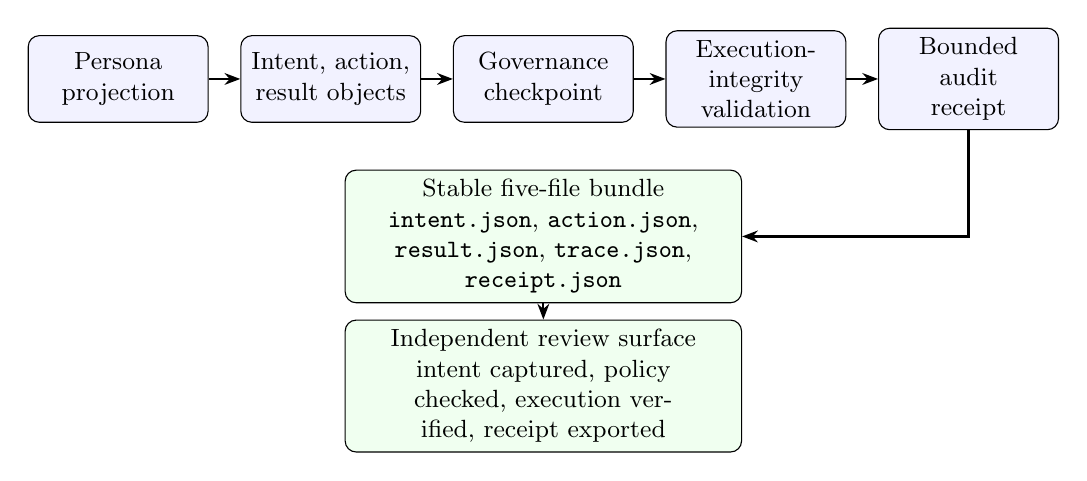
\begin{tikzpicture}[
  box/.style={draw, rounded corners, align=center, text width=2.05cm, minimum height=1.1cm, fill=blue!5, font=\small},
  widebox/.style={draw, rounded corners, align=center, text width=4.8cm, minimum height=1.1cm, fill=green!6, font=\small},
  arr/.style={-{Stealth[length=2mm]}, thick}
]
\node[box] (persona) at (0, 0) {Persona\\projection};
\node[box] (iar) at (2.7, 0) {Intent, action,\\result objects};
\node[box] (gov) at (5.4, 0) {Governance\\checkpoint};
\node[box] (integrity) at (8.1, 0) {Execution-integrity\\validation};
\node[box] (receipt) at (10.8, 0) {Bounded audit\\receipt};
\node[widebox] (bundle) at (5.4, -2.0) {Stable five-file bundle\\\texttt{intent.json}, \texttt{action.json}, \texttt{result.json}, \texttt{trace.json}, \texttt{receipt.json}};
\node[widebox] (review) at (5.4, -3.9) {Independent review surface\\intent captured, policy checked, execution verified, receipt exported};
\draw[arr] (persona) -- (iar);
\draw[arr] (iar) -- (gov);
\draw[arr] (gov) -- (integrity);
\draw[arr] (integrity) -- (receipt);
\draw[arr] (receipt.south) |- (bundle.east);
\draw[arr] (bundle) -- (review);
\end{tikzpicture}
}
\caption{Five-stage architectural view. The controlled evaluation in this paper directly validates the latter four evidence-preserving stages while treating persona projection as an architectural precondition.}
\Description{A five-stage execution evidence pipeline from persona projection through intent, governance, integrity validation, and bounded receipt export into a stable five-file bundle reviewed by four independent checks.}
\label{fig:evidence-architecture}
\end{figure}

\subsection{Reference path}

The architecture is instantiated as a composable reference path in a submitted artifact package omitted here for double-blind review. The implementation keeps the evaluation logic centered in a deterministic local harness so that every condition is reproducible from the included task specifications and scripts.

For every task run, the harness exports exactly five JSON files:

\begin{itemize}
  \item \texttt{intent.json},
  \item \texttt{action.json},
  \item \texttt{result.json},
  \item \texttt{trace.json},
  \item \texttt{receipt.json}.
\end{itemize}

These files are written under the stable layout \texttt{artifacts/runs/<task\_id>/<mode>/}. The contract is shared across all conditions, including baselines and ablations, which makes evidence shape directly comparable.

\subsection{Task suite}

The evaluation harness includes 16 machine-readable tasks grouped into five categories:

\begin{itemize}
  \item four read-only query tasks,
  \item four tool-call tasks,
  \item three budget-constrained tasks,
  \item three approval-required tasks,
  \item two tamper scenarios.
\end{itemize}

The mix of task classes is important because an evidence architecture should represent both positive and negative execution paths. In particular, the budget, approval, and tamper tasks test whether blocked and invalid runs appear as explicit outcomes rather than as absent output.

\subsection{Experimental conditions}

We evaluate ten experimental conditions: a local trace-oriented baseline; two minimal live framework baselines (\texttt{external\_baseline} for CrewAI and \texttt{langchain\_baseline} for LangChain); two same-framework wrapped paths that preserve the live runtime while adding the evidence layer; the full evidence-chain condition; and four single-stage ablations (\texttt{no\_intent}, \texttt{no\_governance}, \texttt{no\_integrity}, and \texttt{no\_receipt}). The live framework baselines preserve framework-native execution evidence but not explicit governance, integrity, or receipt semantics. The paired wrapped modes isolate the effect of the evidence layer while holding the underlying runtime fixed.

\subsection{Review logic and metrics}

A third-party review script consumes a run directory and answers four yes/no questions:

\begin{enumerate}[leftmargin=1.8em]
  \item was intent captured,
  \item was policy checked,
  \item was execution verified,
  \item was a receipt exported.
\end{enumerate}

The script emits machine-readable verdicts, an overall status, missing-field explanations, and a short summary. It also recomputes bundle identity consistency and stored digests rather than trusting exported status labels alone. This review step operationalizes the minimum independent inspection workflow that the architecture is intended to support.

We compare conditions using five deterministic, rule-based metrics derived from actual generated artifacts:

\begin{itemize}
  \item \textbf{explicitness}: whether intent, policy, and outcome are directly inspectable;
  \item \textbf{replayability}: whether the run preserves enough structure for replay-oriented checking;
  \item \textbf{tamper sensitivity}: whether integrity-relevant violations appear as explicit outcomes;
  \item \textbf{audit boundedness}: whether the review surface is compact and purpose-oriented;
  \item \textbf{evidence-stage exposure}: how completely the harness exposes the intended evidence stages (field name: \texttt{integration\_surface}).
\end{itemize}

Some parts of these metrics are directly measurable from the exported fields, while others are scored by transparent 0--5 rules documented in the submitted artifact package. The method does not report semantic-quality scores or invented empirical values.

\section{Evaluation Setup}
\label{sec:evaluation}

All measurements in this draft come from the submitted artifact package. The evaluation asks whether execution evidence should be treated as a distinct systems layer rather than as an extension of runtime logging. The task suite is intentionally heterogeneous: read-only and tool-call tasks cover ordinary successful runs, budget and approval tasks exercise policy gating, and tamper scenarios exercise integrity-sensitive outcomes. Because the same 16 task specifications are used in every condition, score differences are attributable to the exported evidence surface rather than to different workloads.

The review script distinguishes among several outcome classes. A run may be marked \emph{pass} when all four evidence questions are satisfied, \emph{policy\_blocked} when a checkpoint blocks the task but still leaves reviewable evidence, \emph{tamper\_detected} when the integrity layer detects mismatch, or \emph{partial} when one or more evidence-chain capabilities are missing. In the full evidence chain, the artifact summaries show 11 review-passing completed runs, 3 policy-blocked runs, and 2 tamper-detected runs across the 16-task suite.

\subsection{Falsification checks}

To reduce the risk that the review contract merely accepts the study's own positive cases, the artifact package also derives an eight-scenario falsification suite from previously reviewable bundles. Seven scenarios begin from the 11 evidence-chain bundles that the review script already marks as \emph{pass}; the eighth (\texttt{policy\_bypass\_claim}) begins from the 3 evidence-chain bundles that originally reviewed as \emph{policy\_blocked}.

Single-surface removals such as missing intent and missing policy are rebound so that the mutated bundle stays internally consistent except for the targeted capability. Receipt forgery, payload tampering, cross-run replay mismatch, and cross-bundle receipt swap exercise strengthened bundle-identity and digest-binding checks rather than trusting stored status fields. The policy-bypass claim scenario exercises cross-file coherence directly by rewriting a blocked bundle to claim successful completion while leaving the persisted blocked policy decision in place. These checks are reported separately from the main baseline and ablation comparisons because they do not measure runtime quality; they measure whether the independent review contract can reject internally contradictory or transplanted artifacts.

\section{Results}
\label{sec:results}

\subsection{Baseline versus full evidence chain}

Table~\ref{tab:main-comparison} reports the main baseline comparison. The full evidence chain improves every measured dimension over the trace-oriented baseline. Intent capture, policy checking, and receipt export all move from zero observed positive reviews in the baseline to 16 of 16 tasks in the evidence chain. The repository metric records \emph{execution verified} as 11 of 16, but that count should be read in two layers: among the 13 runs that reached the execution stage, 11 completed with verification success and 2 ended as explicit tamper-detected outcomes; the remaining 3 tasks are reviewable policy-blocked outcomes rather than missing bundles.


\begin{table}[t]
\centering
\caption{Trace-oriented baseline versus full evidence chain. Counts report positive bundle-review verdicts across the 16-task suite; scores are average rule-based metrics on a 0--5 scale.}
\label{tab:main-comparison}
\small
\resizebox{\linewidth}{!}{%
\begin{tabular}{lccccccccc}
\toprule
Mode & Intent & Policy & Exec.\ verified & Receipt & Explicitness & Replayability & Tamper & Audit & Integration \\
\midrule
    Baseline & 0/16 & 0/16 & 0/16 & 0/16 & 1.0 & 3.0 & 0.0 & 2.0 & 1.0 \\
    Evidence chain & 16/16 & 16/16 & 11/16 & 16/16 & 5.0 & 5.0 & 4.81 & 5.0 & 5.0 \\
\\
\bottomrule
\end{tabular}%
}
\end{table}


The metric changes are large. Average explicitness rises from 1.0 to 5.0, replayability from 3.0 to 5.0, tamper sensitivity from 0.0 to 4.81, audit boundedness from 2.0 to 5.0, and evidence-stage exposure from 1.0 to 5.0. This pattern supports the paper's narrower claim: within a stable exported-bundle contract, the evidence-chain surface preserves review questions that the trace-oriented surface does not explicitly retain.

\subsection{External baseline comparison}

Table~\ref{tab:external-comparison} compares the minimal live CrewAI baseline with the full evidence chain. The external baseline improves replayability relative to the local baseline, reaching an average score of 4.0, because a real CrewAI runtime now produces the task execution surface that is later normalized into the five-file bundle. However, it still leaves explicit intent capture, policy persistence, integrity verification, and receipt export absent. As a result, explicitness, tamper sensitivity, audit boundedness, and evidence-stage exposure remain at 1.0, 0.0, 2.0, and 1.0 respectively.


\begin{table}[t]
\centering
\caption{CrewAI-like external baseline versus the full evidence chain. The external baseline preserves a richer default execution surface than the local trace baseline, but does not add explicit evidence-chain semantics.}
\label{tab:external-comparison}
\small
\resizebox{\linewidth}{!}{%
\begin{tabular}{lccccccccc}
\toprule
Mode & Intent & Policy & Exec.\ verified & Receipt & Explicitness & Replayability & Tamper & Audit & Integration \\
\midrule
    External baseline & 0/16 & 0/16 & 0/16 & 0/16 & 1.0 & 4.0 & 0.0 & 2.0 & 1.0 \\
    Evidence chain & 16/16 & 16/16 & 11/16 & 16/16 & 5.0 & 5.0 & 4.81 & 5.0 & 5.0 \\
\\
\bottomrule
\end{tabular}%
}
\end{table}


This comparison only partially addresses the straw-baseline concern. Because the baseline is a minimal live integration rather than a full production benchmark, the result should be read as evidence that a framework-native default logging surface still leaves major evidence gaps by default, not as a definitive benchmark against every production framework.

\subsection{Ablation results}

Table~\ref{tab:ablation-comparison} summarizes the seven-mode comparison. The ablations show targeted degradation rather than uniform collapse.


\begin{table}[t]
\centering
\caption{Seven-mode comparison across the baseline, external baseline, four ablations, and the full evidence chain. Scores are average 0--5 values; counts report positive review verdicts across 16 tasks.}
\label{tab:ablation-comparison}
\small
\resizebox{\linewidth}{!}{%
\begin{tabular}{lccccccccc}
\toprule
Mode & Explicitness & Replayability & Tamper & Audit & Stage exposure & Intent & Policy & Exec.\ verified & Receipt \\
\midrule
    Baseline & 1.0 & 3.0 & 0.0 & 2.0 & 1.0 & 0/16 & 0/16 & 0/16 & 0/16 \\
    External baseline & 1.0 & 4.0 & 0.0 & 2.0 & 1.0 & 0/16 & 0/16 & 0/16 & 0/16 \\
    No intent & 3.0 & 4.0 & 4.81 & 4.0 & 4.0 & 0/16 & 16/16 & 11/16 & 16/16 \\
    No governance & 2.0 & 5.0 & 5.0 & 4.0 & 4.0 & 16/16 & 0/16 & 14/16 & 16/16 \\
    No integrity & 5.0 & 5.0 & 0.0 & 5.0 & 4.0 & 16/16 & 16/16 & 0/16 & 16/16 \\
    No receipt & 4.0 & 4.0 & 4.81 & 2.0 & 4.0 & 16/16 & 16/16 & 11/16 & 0/16 \\
    Evidence chain & 5.0 & 5.0 & 4.81 & 5.0 & 5.0 & 16/16 & 16/16 & 11/16 & 16/16 \\
\\
\bottomrule
\end{tabular}%
}
\end{table}


Removing intent capture lowers explicitness from 5.0 to 3.0 and evidence-stage exposure from 5.0 to 4.0, while leaving policy, integrity, and receipt behaviors mostly intact. Removing governance lowers explicitness to 2.0, eliminates all positive policy-checked reviews, and changes the task suite behavior by allowing formerly blocked tasks to complete, while tamper sensitivity remains high because integrity checks are still present. Removing integrity leaves explicitness and audit boundedness at evidence-chain levels, but drives tamper sensitivity and execution verification to 0.0 and 0 of 16. Removing receipt export preserves most other capabilities but drops audit boundedness from 5.0 to 2.0 and receipt-exported reviews from 16 of 16 to 0 of 16.

Taken together, the ablations indicate that each stage contributes a distinct review function. The evidence chain therefore behaves as a layered architecture rather than as a single monolithic switch.

\subsection{Human-review scaffold}

The blinded human-review kit is retained as workflow infrastructure rather than as a main empirical result. Because the checked-in sheet is synthetic, the paper does not use those values as evidence of usability or reviewer performance. We therefore treat the human-review component as protocol readiness only and defer the smoke-test details to Appendix~\ref{sec:appendix-human-review}.

\section{Related Work}

This work sits at the intersection of runtime observability, provenance and audit modeling, policy enforcement, and agent-framework execution tooling. The paper does not attempt to replace those lines of work. Instead, it argues that agentic software systems need an additional bridge layer that turns runtime traces into bounded evidence bundles for independent review.

Runtime observability systems standardize logs, metrics, and traces as the primary surface for inspection. OpenTelemetry is representative of this design center \cite{opentelemetry}, while framework-specific tooling such as LangSmith observability and CrewAI tracing exposes agent traces, callbacks, and task timelines for debugging and operations \cite{langsmith-observability,crewai-tracing}. These systems make runs inspectable, but they do not by default provide a review contract that explicitly preserves intent capture, policy persistence, integrity status, and receipt export.

Provenance research emphasizes lineage, responsibility, and reproducibility across heterogeneous systems. PROV-O remains a foundational provenance vocabulary for interoperable provenance interchange \cite{prov-o}, and recent work such as PROV-AGENT extends this tradition to agentic workflows by capturing prompts, responses, and decisions as workflow provenance \cite{prov-agent}. Our execution-evidence layer is narrower than full provenance graphs: it compresses the run into a bounded bundle designed specifically for third-party review questions.

Policy systems show that authorization can be externalized and made explicit. Open Policy Agent is a widely used example of policy-as-code infrastructure \cite{opa}. Recent receipt-oriented work also argues that lightweight execution receipts can offer a practical middle ground between unstructured logs and heavyweight cryptographic proof systems for interactive agents \cite{tool-receipts}. The present paper adopts that general intuition, but evaluates it at the level of exported run bundles, review logic, and controlled architectural ablations.

Relative to these strands, the claim of this paper is modest. Observability surfaces, provenance models, and policy engines each solve part of the problem, but they do not automatically yield an evidence bundle that a third party can inspect without reconstructing the original runtime context. The proposed architecture is intended as that missing bridge, not as a replacement for tracing, provenance, or policy tooling.

\section{Discussion and Threats to Validity}
\label{sec:discussion}

The reported results support a bounded systems claim: execution evidence can be modeled as a distinct layer above runtime observability and below downstream audit interpretation. In the implemented harness, this layer improves pre-execution explicitness, preserves governance outcomes as evidence-bearing states, detects tamper scenarios as explicit review results, exports bounded receipts that a third party can inspect without reading a full trace transcript, and rejects falsified bundle variants derived from previously valid runs.

The results do not show semantic correctness of model outputs, formal verification of arbitrary agent behavior, or a complete representation of any production framework. The paper should therefore be read as a reference-architecture and reference-implementation study, not as a claim of universal runtime coverage.

Threats to validity remain. The metrics are evidence-shape metrics rather than semantic task-quality metrics. The harness is deterministic and local, so it does not exercise the nondeterminism, service failures, and integration drift of production agent stacks. The live framework baselines are minimal integrations, not production benchmarks, although the paired CrewAI and LangChain comparisons materially reduce the straw-baseline concern. The falsification suite also remains bounded: it strengthens adversarial validity by checking omission, replay mismatch, receipt swap, policy-bypass claims, payload tampering, and false tamper claims, but it does not cover open-ended attacks or broader live-service adversaries. Persona projection likewise remains the least validated stage and is treated here as an architectural precondition rather than an independently established causal factor.

Despite these limits, the reference path is useful for software engineering practice. It suggests that agentic systems need a distinction between \emph{runtime telemetry}, which helps operators observe a system, and \emph{execution evidence}, which helps reviewers verify what the system claimed to do.

\section{Conclusion}

This paper presented an execution evidence architecture for agentic software systems and instantiated it as a reproducible reference path in an artifact package omitted here for double-blind review. The central claim is that observability alone is not enough: agent runs need structured evidence bundles that make intent, authorization, execution verification, and exported receipts independently reviewable.

The checked-in evaluation harness supports a bounded version of that claim with a deterministic 16-task suite, a stable five-file export contract, a third-party review script, minimal live CrewAI and LangChain baselines, paired same-framework comparisons in both frameworks with and without the evidence layer, four ablation modes, and a small negative-control falsification suite. An appendix-only blinded reviewer workflow is also included as reproducibility scaffolding. Across the current summaries, the full evidence chain preserves review questions that the trace-oriented baseline and the live framework observability baselines do not explicitly retain, the same live runtime becomes reviewable when wrapped by the evidence layer in two framework ecosystems, the architecture shows interpretable degradation under targeted ablations, and the same review contract rejects several malformed or over-claimed bundles derived from previously valid runs.

Future work should validate the architecture against live framework integrations, extend the integrity layer beyond the current bounded checks, and run a real blinded reviewer study. Even in its current form, the reference implementation shows a plausible and reproducible path for engineering execution evidence as a first-class systems layer rather than treating it as a side effect of logging.

\input{sections/data_availability}

\bibliographystyle{ACM-Reference-Format}
\bibliography{refs}

\end{document}
